\documentclass[11pt]{article}
\usepackage{geometry}                % See geometry.pdf to learn the layout options. There are lots.
\geometry{letterpaper}                   % ... or a4paper or a5paper or ... 
%\geometry{landscape}                % Activate for for rotated page geometry
%\usepackage[parfill]{parskip}    % Activate to begin paragraphs with an empty line rather than an indent
\usepackage[pdftex]{graphicx}
\usepackage{amssymb}
\usepackage{epstopdf}

\usepackage[T1]{fontenc}
\usepackage[scaled=0.8]{beramono}

%\DeclareGraphicsRule{.tif}{png}{.png}{`convert #1 `dirname #1`/`basename #1 .tif`.png}
\usepackage{listings} 

\lstset{%
  numbers=none,
  sensitive=true,
  morecomment=[l]{//},
  morecomment=[s]{/*}{*/},
  morestring=[b]",
  emphstyle={\bf},
  commentstyle=\it,
  stringstyle=\mdseries\ttfamily,
  showspaces=false,
  basicstyle=\ttfamily,
  morekeywords={schema,type},
  keywordstyle=\bfseries,
  columns=flexible,
  showstringspaces=false,
  morecomment=[l]\%,
}

\lstdefinelanguage{Schema}{%
  numbers=none,
  sensitive=true,
  morecomment=[l]{//},
  morecomment=[s]{/*}{*/},
  morestring=[b]",
  emphstyle={\bf},
  commentstyle=\it,
  stringstyle=\mdseries\ttfamily,
  showspaces=false,
  basicstyle=\ttfamily,
  morekeywords={class},
  keywordstyle=\bfseries,
  columns=flexible,
  showstringspaces=false,
  morecomment=[l]\%,
}

\newcommand{\C}{\lstinline}

\lstset{language=Ruby}

\newcommand{\Enso}{Ens\={o}}

\title{
\includegraphics[scale=0.25]{enso.jpg}\\  Managed Data:\\ Structure and Interpretation of Data in \Enso}
\author{William R. Cook and Tijs van der Storm}
%\date{}                                           % Activate to display a given date or no date

\begin{document}
\maketitle

\begin{abstract}
Managed Data allow programmers to define or modify the
fundamental data definition mechanisms in a programming language. 
The programmer can change the language used to describe data, implement
that language by writing or modifying interpreters, and
integrate the new data mechanisms with existing language
support for data access and manipulation. For example,
Managed Data allow programmers to override the field/method
access operator (the ``dot operator''). Managed Data allow
easy implementation of many aspects of data, including 
logging/subscription, access/change control, bidirectional 
relationships, invariants and validation.
A bootstrap process is used so that all data, including the
data used to implement Managed Data, is managed.
This paper describes the implementation of Managed Data
as the foundation of \Enso, a new programming system based on 
model interpretation.
\end{abstract}

\section{Introduction}

Mechanisms for organizing and managing data are a fundamental
aspect of any programming model. Most programing models provide
built-in mechanisms for organizing data. Well known approaches 
include \textit{data structure definitions} (as in Pascal, C, Haskell, ML),
\textit{object/class models} (as in Java, Smalltalk, Self), and \textit{predefined
data structures} (as in Lisp, Matlab).
Languages may also support type abstraction (as in ML, Ada), a combination of 
multiple approaches (e.g JavaScript, Scala), or other variations.
The key characteristic of all these approaches is that the
fundamental mechanisms for structuring and manipulating data are 
predefined.
Predefined data structuring mechanisms allow programmers to create
specific kinds of data, but they do not usually allow 
fundamental changes to the underlying data structuring and 
management mechanisms. 

Predefined data structuring mechanisms are insufficient to cleanly
implement many important and common requirements for data management,
including persistence, caching, serialization, transactions, change logging,
access control, automated traversals, 
multi-object invariants, and bi-directional relationships. 
The difficulty with all these requirements is that they are best 
implemented as pervasive features of the underlying data management
mechanism. It is possible to defined such features individually for
each particular kind of data in a program, but this typically leads to
large amounts of repeated code. To implement these kinds of crosscutting
concerns, developers often
resort to preprocessors, code generates, byte-code transformation, 
or modified runtimes or compilers. The resulting systems are typically ad-hoc,
fragile, poorly integrated, and difficult to maintain.

What is involved in making fundamental and potentially pervasive 
changes to the way data is managed in a programming model? There are
several ways to approach this question, but one concrete example is to
consider what it would mean to override the ``dot'' operator, which 
selects a field of a structure or object in many languages. One might also
consider a global override of the field assignment operator. Giving the
programmer control over the data manipulation mechanisms means defining
or modifying the behavior of all the data manipulation operations that
are often considered built-in primitives, including initialization, type tests, 
casting, pointer equality, and field access. In this view, the
data structuring mechanisms are an \textit{aspect} of an overall programming
system. 

Some programming systems support a degree of control over 
the data structuring mechanisms. Meta-classes in Smalltalk define how
classes are instantiated and compiled. 
The reflective features of Ruby, Python and Smalltalk 
can be used to trap and handle undefined methods and properties, 
which can be used to create proxies or implement virtual objects.
Scheme macros are often used to create data structuring mechanisms.
For example, the \lstinline{defstruct} macro defines mutable structures
with a functional interface. However... <summarize>. 
The Adaptive Object Model Architecture provides an architecture for
this approach, but does not discuss how it is bootstrapped or integrated
with existing languages.

This paper presents Managed Data, an approach to data definition
in which programmers have control over the data structuring 
mechanisms, either to define
new mechanisms or modify the system's built-in mechanisms. 
Managed Data has four main features: (1) high-level data models,
called \textit{schemas},
that specify the structure and behavior of data, 
(2) \textit{data managers} that interpret schemas and that manage data instances, 
(3) \textit{programming language integration} so that managed instances
can accessed just like normal data,
and (4) a \textit{bootstrapping} process
that allows all Managed Data, including data models, to be customized
and managed. Managed Data
places strong requirements on the host programming language, to 
support use-defined interpretation of data.

In this paper we illustrate the concept of Managed Data in an object-oriented
style. It is also possible to imagine implementations for other
programming styles, including functional or logic programming. Some of
these options are discussed further in Section~\ref{discussion}.

\section{Examples}

This section gives examples of using and implementing Managed Data.

\begin{figure}[language=Schema]
\begin{minipage}{0.5\columnwidth}
\begin{lstlisting}
class Machine
  start: State
  states: State*

class State
  machine: Machine / Machine.states
  name: str
  out: Transition*
  in: Transition*
  
class Transition
  event: str
  from: State / State.out
  to: State / State.in
\end{lstlisting}
\end{minipage}
\begin{minipage}{0.5\columnwidth}
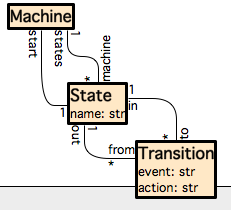
\includegraphics[scale=0.9]{state_machine.png}
\end{minipage}
\caption{A schema for simple state machines}
\label{sm_schema}
\end{figure}

\subsection{Using Managed Data}

Managed Data allows a programmer to 
build libraries, or \textit{data managers}, that implement the fundamental
data manipulation primitives in a programming language. 
The input to a data manager is a \textit{schema},
which describes the structure and behavior of the data to be managed.
Although there can be many flavors of schemas and data managers in a 
Managed Data system, it is useful to illustrate the concepts using a
specific example. This section presents illustrates schemas and
the creation and use of managed data instances. Following sections will 
describe how to implement data managers and integrate them with programming
languages. 

Figure~\ref{sm_schema} defines a schema for a simple form of
state machine. The schema consists of three \textit{classes}, for
state machines, states, and transitions. The body of a class definition
is a list of \textit{fields} of the form \textit{name}\lstinline{:}\textit{type}, where \textit{type}
is either a class name or one of the primitive types (\lstinline{int}, \lstinline{str}, \lstinline{bool}). 
The field definition is followed by some attributes. The suffix 
\lstinline{*} after the name means
that the field is multi-valued.
For example, the \lstinline{Machine}
class has two fields, a \lstinline{start} state and a 
multivalued field \lstinline{states} containing a set of states.
A class-valued field may also have an \textit{inverse}. For example,
the \lstinline{machine} field of the \lstinline{State} class is the
inverse of the \lstinline{states} field in the \lstinline{StateMachine} class.
A field and its inverse are semantically tied. For example, setting the
\lstinline{machine} field of a state causes the state to be added to the
\lstinline{states} collection of the machine. In general, any change to
\lstinline{states} or \lstinline{machine} requires a corresponding change 
to the other field of the related object.
The concept of inverse fields is frequently used in object-relational
mapping. 

\begin{figure}[t]
\begin{lstlisting}
state_machine_schema = Load("state_machine.schema")
f = InMemoryDataManager.new(state_machine_schema)

# create the state machine, by calling constructors of the factory
door = f.Machine                # create the door state machine
open = f.State(door, "Open")     # create and add the open state to the door
closed = f.State(door, "Closed")                   # create and add the closed state to the door
f.Transition("close", open, closed)  # create a transition from open to closed
f.Transition("open", closed, open)              # create a transition from closed to open
door.start = open         # set the start state of the machine
door.validate             # validate the state machine graph, checking invariants

run_state_machine(door)    # run the machine (see next figure)
\end{lstlisting}
\caption{Creating a simple state machine using an in-memory data manager}
\label{sm_create}
\end{figure}

A schema defines the structure and behavior of data. The simple schema
for state machines is primarily structural, but it does include some
behavioral constraints, in the form of field inverses. More complex schemas
can include invariants, constraints, computed fields, database information,
or other kinds of meta-data. Several of these options are described in later
sections. 

Once a schema is written, it can be loaded into a data manager to
create and manage instances of classes defined in the schema. 
There is no need for an additional code generation step to
translate the schema into code. 
Instead, a data manager interprets the schema directly, and
creates dynamic objects that act according to the specification of the
schema, but without needing to write any more code. 
The data manager can then be used instantiate objects, which are
given fields (and behaviors) as defined in the schema.

Figure~\ref{sm_create} illustrates using the state machine schema
to create a simple state machine for a door. The \lstinline{Load}
function loads objects from a file, in this case it loads the
schema defined in Figure~\ref{sm_schema}. 
The \lstinline{InMemoryDataManager} is a particular data manager
that manages in-memory objects. The \lstinline{InMemoryDataManager}
is passed a schema as an input and returns a \textit{factory}.
The factory \lstinline{f} has dynamically defined methods for each class in the
schema. For example, the methods \lstinline{f.Machine} and 
\lstinline{f.State} create machines and states, respectively.
These constructor functions take an arbitrary number of arguments,
which are used to initialize the fields (in order) of the class.
The \lstinline{f.Machine} call just creates a state machine with
no intialization. The \lstinline{f.State(sm, "Open")} call creates
a state, initializing its \lstinline{machine} and \lstinline{name} fields.
As mentioned above, setting the \lstinline{machine} of a state has the 
side effect of adding the state to the machine's \lstinline{states} collection.
A state machine can also be read from a file, using a parser and a 
state machine grammar.

Once the machine is created, it is validated. In this case validation
means that the machine is checked for consistency and then locked, so
that it cannot be changed. The semantics of validation is determined
by the particular data manager that is used. 

A data manager works very much like a
relational database management system (RDBMS), 
where the SQL Data Definition Language (DDL) defines a schema. 
The RDBMS interprets the schema to create tables, which can then
be accessed in SQL queries. 
Managed Data imports this approach from databases into
the core of a programming language. 

\begin{figure}[t]
\begin{lstlisting}
# this function runs a state machine, by reading events from an input stream
def run_state_machine(sm)
  current = sm.start   # access the start state of the state machine
  puts current        # print the current state
  while gets               # read a line of input and check for end of file
    input = $_.strip   # capture the input line
    current.out.each do |trans|   # iterate over each outgoing transitions
      if trans.event == input            # test of the transition event equals the input
        current = trans.to               # if so, change to the new state
      end
    end
    puts current.name  # print the current state (which may not have changed)
  end
end
\end{lstlisting}
\caption{A function to interpret a state machine}
\label{sm_run}
\end{figure}

Managed Data also 
drops the idea of a single predefined schema language, and
allows programmers to create their own 
(or variations on existing) schema languages and schema managers.
Data managers naturally manage many schemas, but 
there can also be multiple data managers for a given 
schema, for example, to implement in-memory strategy versus
a database strategy for managing the data. 

Finally, the machine is run. The code for running a state machine is
given in Figure~\ref{sm_run}. At this point the dynamic state machine object
\lstinline{sm} is treated just like any other object. It has a field 
named \lstinline{start} that is directly accessed using dot notation. 
The \lstinline{current} variable is a state object, which has a fields
\lstinline{name} and \lstinline{out}, which is a collection of transitions, 
which have fields \lstinline{event} and \lstinline{to}.

\subsection{Implementing Managed Data}

The example usage illustrated in the previous section cannot
be implemented easily in most programming languages. In many
object-oriented languages (e.g. Java, C\#, JavaScript, and PHP) 
the dot operator, which is used to access
fields \lstinline{o.f} and methods \lstinline{o.m(args)},
requires a declared class or record that defines 
a field \lstinline{f} or a method \lstinline{m}. 
But the example in the previous section requires dynamic
definitions of fields and methods: the factory implements methods 
based on the classes listed in the metadata object, and the
objects created by the factory contain fields that are specified
in a schema.
To get around this problem, most approaches to model-driven 
development resort to code generation.  However, our approach
is based on dynamic interpretation, so alternative techniques
are required.

\begin{figure}
\begin{lstlisting}
class RecordManager
  def initialize(types)
    @types = types
    @values = {}
    puts types
    types.each_pair do |key, type| 
      @values[key] = type.default
    end
  end
  def method_missing(name, *args)
    assign = (name =~ /(.*)=/)
    name = $1.to_sym if assign
    raise "unknown field #{name}" if !@types[name]
    if assign
      raise "#{name} must be #{@types[name]}" if @types[name] != args[0].class
      @values[name] = args[0]
    else
      return @values[name]
    end
  end
end
\end{lstlisting}
\caption{Definition and use of a simple data manager in Ruby}
\label{sdm}
\end{figure}

In what follows, we used the reflective capabilities
found in some object-oriented languages, including Smalltalk, Ruby,
and Python, to implement Managed Data.
In Ruby the form \lstinline{o.f}
can be implemented by defining a \lstinline{method_missing} method.
This technique is illustrated in 
Figure~\ref{sdm}, which defines a simple data manager for 
updatable records, using Ruby.
This data manager is simpler than the one used in in the previous
section, but it illustrates the basic technique.
As in the previous section, the data manager is initialized with
a schema, but in this case the schema is a record of types rather than
a full data model. The managed object stores the type record in the
\lstinline{@types} member variable. It then defines a \lstinline{@values}
record and initializes it with default values for each type (the way
that default values are defined is omitted). 

Here is an example using the record manager:

\begin{lstlisting}
x = RecordManager.new :foo => Fixnum, :bar => String
puts x.foo
x.foo = 32
x.biff            # throws undefined field
x.foo = "asdf"    # throws a type exception
puts x.foo
\end{lstlisting}

The key mechanism for implementing a dynamic object is the 
\lstinline{method_missing} method. It is called whenever a method (or field)
is called on the object that is not defined. Since the class does not
define any methods, the \lstinline{method_missing} is called for all fields
and methods. The arguments to \lstinline{method_missing} are the method
name and the arguments of the original call. There is one special case. 
In Ruby, an assignment to a field,
of the form \lstinline{obj.field = val} is converted into a  
call of the form \lstinline{o.method_missing(:field=, val)}, where
\lstinline{:field=} is a symbol formed by appending \lstinline{=} to the
field name.

The \lstinline{method_missing} method first checks if the call is a 
field assignment, in which case it sets \lstinline{assign} to true. 
If it is an assignment, the field name is updated to remove the \lstinline{=}.
It then checks if the field is defined in the schema, and returns an 
error if not. For an assignment, it checks if the argument is 
of the right type, and raises an error if not. It then updates the
\lstinline{@values} map with the new value. For regular field access,
it returns the current value for the named field in \lstinline{@values}.

\begin{figure}
\begin{lstlisting}[language=Schema]
class Schema
! types: Type*

class Type
# name: str
  schema: Schema / Schema.types

class Primitive < Type
  
class Class < Type
  supers: Class*
  subclasses: Class* / Class.supers
! defined_fields: Field*
  fields: Field* = "supers.flat_map(&:fields) + defined_fields"
  
class Field
# name: str
  owner: Class / Class.defined_fields
  type: Type
  optional: bool
  many: bool
  key: bool
  inverse: Field? / Field.inverse 
  computed: str?
  traversal: bool

primitives str, int, bool, real
\end{lstlisting}
\caption{The Schema of Schemas}
\label{schema_schema}
\end{figure}

\section{Schemas}

%<alex-comment: is it better to talk about a normal schema first and introduce the Schema schema later? Might be confusing here. And it is easier to argue why the Schema-schema is important and what cool things you can do with it once the big picture is obvious />

While there are many kinds of schemas and data managers in \Enso,
there is one basic schema, the Schema Schema, that is used in the implementation of
\Enso\ itself. The goal of a Schema Schema is to be rich enough to describe useful
data and be self-describing w
hile still small enough to act as a kernel language of schemas.
The Schema Schema we have designed for \Enso\ is certainly not as
minimal as possible, but it is still simpler than UML MOF, for
example.

Figure~\ref{schema_schema} defines the Schema Schema in \Enso. 
A \lstinline{Schema} has a collection of \lstinline{types}. 
The \lstinline{!} annotation indicates that \lstinline{types}
is a \textit{traversal} field. Traversal fields defined a spanning tree
in the graph, which can be used to visit every node in the graph efficiently.
Traversal fields are also used for naming.
A \lstinline{Type} has a \lstinline{name} and a reference
to the \lstinline{schema} that it belongs to (defined as the inverse of the
\lstinline{Schema.types} field, as discussed in Section~\ref{inverse}).
The \lstinline[language=Schema]{#} annotation indicates that the \lstinline{name} field
is a \textit{key} field within any collection of types. This ensures that
no two types have the same name.

The two subclasses of \lstinline{Type} are 
primitive types and class definitions. A primitive has
no additional fields. A class has a set of super classes and
subclasses. The \lstinline{subclass} field is the inverse of the \lstinline{supers} field.
A class has a set of \lstinline{defined fields}, which are the fields that
are directly defined in the class. Classes also have a computed field, \lstinline{fields},
which implements inheritance. The \lstinline{fields} of a class are computed as
the sum of the fields of all superclasses, combined with the defined fields of the class.
The expression that implements a computed field is currently quoted Ruby code,
although future versions of \Enso\ will have a DSL for computed field expressions.

A \lstinline{Field} has a \lstinline{name} and a \lstinline{type} and an \lstinline{owner}.
The \lstinline{owner} is the class that defines the field (i.e. the inverse of \lstinline{Class.defined_fields}).
The \lstinline{type} is the \lstinline{Type} of the value of the field.
Boolean flags are used to identify the field as \textit{optional}, \textit{many valued},
\textit{key}, and \textit{traversal}. An optional \lstinline{computed} field defines the
expression for computing the field. A field also has an optional \lstinline{inverse}, 
which, interestingly enough is its own inverse.

Some invariants (why aren't these in the schema?):
\begin{lstlisting}
  !f.inverse.nil? => f.inverse.inverse = f
  !f.inverse.nil? => f.inverse.owner = f.type
  !f.inverse.nil? => f.inverse.type = f.owner
  f.key => !f.many && !f.optional && f.type.Primitive?
\end{lstlisting}
  
The \textit{traversal} fields in a schema have a special role. <MORE>

Constraints


\subsection{Modularity}

talk about merging schemas!!

\section{Data Managers}

Structure are created by \textit{factories}, which create
and manage the nodes in the structure. The factory also
ensures that structures are distinct: a factory identifies the 
collection of nodes that belong to a graph, and any given node 
can only be connected to other nodes in the same graph, which were
created by the same factory.

In \Enso\ most properties of a structure are
checked when the structure is being created. In other words, 
the \textit{factory} that creates the structure is parameterized by a
schema, which the factory uses to check the legality of operations
on the objects it creates.

\begin{figure}[t]
\begin{lstlisting}
class Factory
  def initialize(schema)
    @schema = schema
  end

  # factory.Class(args) creates an instance of Class initialized with arguments  
  def method_missing(name, *args)
    klass = @schema.classes[name.to_s]
    raise "Unknown class '#{name}'" unless klass
    obj = CheckedObject.new(klass, self)
    klass.fields.each_with_index do |field, n|
      if n < args.length  # if there is an initializer
        if field.many     # add items for many-valued fields
          args[n].each { |x| obj[field.name] << x }
        else              
          obj[field.name] = args[n]  # else initialize the field
        end
      elsif !field.key && !field.optional && field.type.Primitive?
        obj[field.name] = field.type.default   # initialize required primitive fields
      end
    end
    raise "too many initializers in #{name}(#{args})" if n < args.length
    return obj # return the new object
  end
end
\end{lstlisting}
\caption{Data manager for any schema}
\label{sm_run}
\end{figure}


\begin{figure}[t]
\begin{lstlisting}
class CheckedObject 
  def initialize(schema_class, factory) #, many_index, many, int, str, b1, b2)
    @schema_class = schema_class
    @values = {}
    schema_class.fields.each do |field|
      continue if !field.many
      if (key = ClassKey(field.type))
        @values[field.name] = ManyIndexedField.new(key.name, self, field)
      else
        @values[field.name] = ManyField.new(self, field)
      end
    end
  end

  def method_missing(m, *args)
    (m =~ /(.*)=/) ? (self[$1] = args[0]) : self[m.to_s]
  end
  
  def [](name)
    if name[-1] == "?"
      name = name[0..-2]
      return Subclass?(@schema_class, @schema_class.schema.types[name])
    end
    field = @schema_class.fields[name]; 
    raise "Accessing non-existant field '#{name}'" unless field
    return field.computed ? instance_eval(field.computed) : @values[name]
  end

  def []=(name, new)
    field = @schema_class.fields[name]
    raise "Assign to invalid field '#{name}'" unless field
    raise "Can't assign field '#{name}'" if field.computed || field.many
    raise "Can't clear required field '#{name}'" if new.nil? && !field.optional
    check_type field.type, new
    old = @values[name]
    return new if old == new
    @values[name] = new
    notify_update(field, old, new)
    return new
  end
\end{lstlisting}
\caption{Checked object implements dynamic object conforming to schema class}
\label{sm_run}
\end{figure}

\subsection{Graph Ownership}

The programming model is based on cyclic graphs.
Graphs are kept distinct from each other. That is,
each graph is considered a self-contained
artifact, without links or pointers to other graphs.

\subsection{Maintaining Inverses}

\subsection{Preserving Order}

\subsection{Dynamic Updates}

\subsection{Listeners}

\subsection{Instance Modification}

change tracking

Managed Data supports controlled imperative effects. Objects are
mutable during construction or modification, while the data may be in an
inconsistent state, but before it can be used it must be validated
and locked from further changes. This is similar to a transaction.


\subsection{Differences}


\subsection{Instantiation}


\section{Bootstrapping}


\subsection{QuadModel}

%<alex
%Quad Model
%AKA Self-describing meta-models

%-*** Not sure if it is really a 'quad' model as this paper does not 
% introduce the notion of a grammar or any other presentation
% model ***

%0) Introduce grammar????
%- Or just present a recursive 'stack' model?

%2) WHY do we want this (the beginning)
%- Schemas are also data
%  - we need to describe data
%  - we want flexibility in how data is organized

(In order to ...)
(we need ... expose data structuring ... to programmers)
(how is this a problem in other languages that support meta-programming? eg smalltalk) 

%1) WHAT is it
%- schema are data
%  - schema-schema
%  - self-describing 
%  - similar to ER diagram
%  - explicitly specified 
%  - and can be changed
%= analogous to the self-conforming meta-meta-model in MDE or Class class in Smalltalk
One of the key features of \Enso\ is that schemas are modeled as data, complete with their own "schema of schemas" which describes how all schemas are organized, including itself. The schema of schema is (similar to ER diagram, rationale for design...)

Like any other data definitions, the schema schema is not hardcoded but explicitly specified, allowing it to be extended or modified. This allows the programmer to alter the data structuring mechanism in very fundamental ways. An immediate use case is to refine the schema schema for different data managers. For instance, a database manager might expect the schema to hold information about mappings between classes and tables, maximum text sizes, and primary keys, on top of the entity-relationship model. A relational database may also preclude many-to-many relationships between entities. Both the constraints and extra information can be encoded naturally by augmenting the schema schema with new attributes and invariants to Fields.

<add picture of how the schema schema can be refined?>

%4) More cool stuff we can do with it
%- add more levels
%  - eg?
%- modify the base 
%  - eg DB needs table name
%  - what else?

The editable and recursive nature of the schema meta-stack means that the way data is defined can be changed in very fundamental ways.

%- reuse tools at meta level
Yet another benefit of the congruence between data and schema is that the same support tools such as editors and formatters can be used both when designing schemas and specifying their data. Not only will we have one less set of tools to build, but programmers also face lower hurdles when learning /Enso/.

% 3) HOW do we do it
TODO ... Something about bootstraps


%/alex>

\begin{figure}[htbp]
\begin{center}
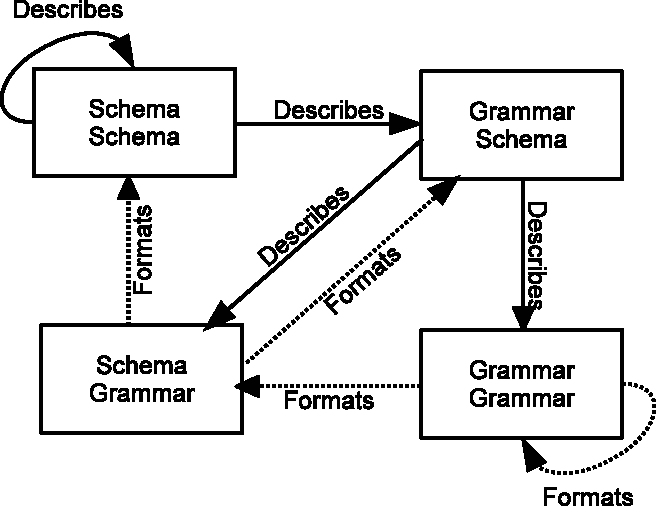
\includegraphics[scale=0.7]{QuadModel.pdf}
\caption{The four core schema and grammar models}
\label{default}
\end{center}
\end{figure}


\begin{figure}
\begin{center}
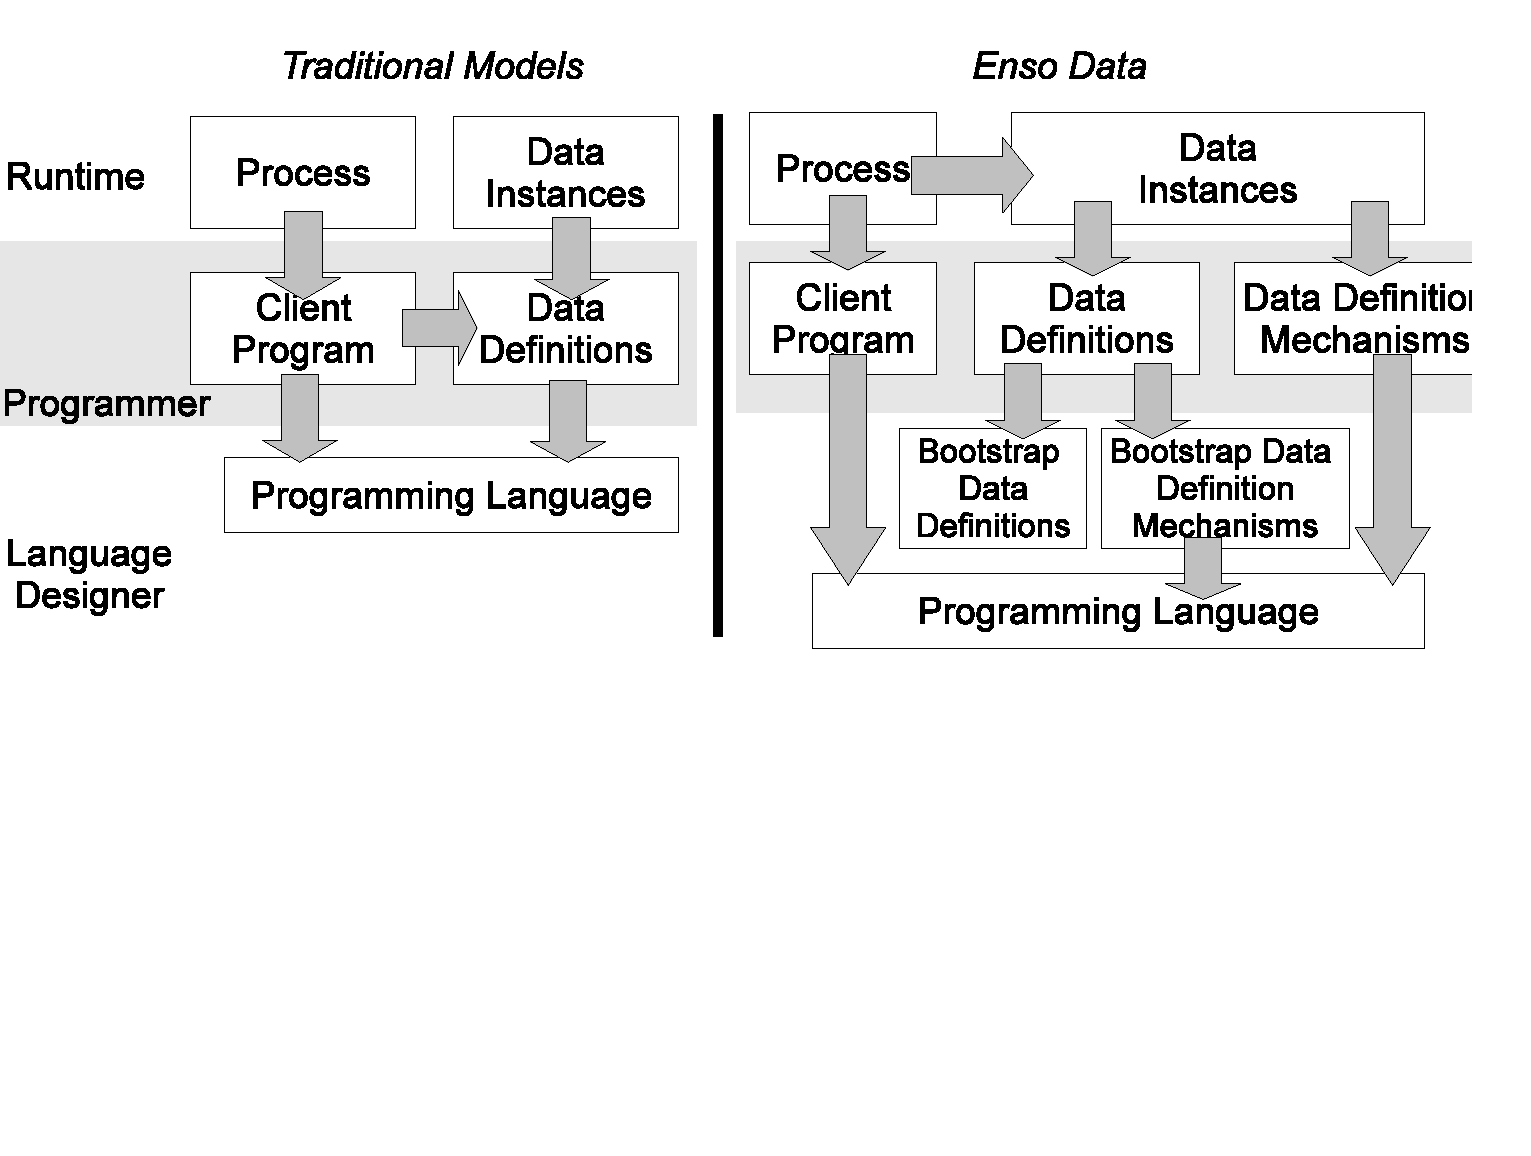
\includegraphics[scale=0.5]{DDL.pdf}
\caption{Traditional versus Managed data definitions}
\label{ddl}
\end{center}
\end{figure}

\section{Discussion}

Figure~\ref{ddl} illustrates the difference between 
traditional built-in data structuring mechanisms and Managed Data.
In the traditional approach, the programming language includes a 
process and data sublanguages, which are both predefined.
With Managed Data, the data structuring mechanisms are defined
by the programmer by interpretation of data definitions.
Since a data definition model is also data, it requires a meta-definition
mechanism. This infinite regress is terminated by a boot-strap
data definition that is used to build the Managed Data system itself.

One more subtle issue is what organizational principle to use for
structuring data. 
Two obvious options are \textit{trees} or \textit{graphs}. Trees are
frequently used in functional languages and are appealing because
of their strong support for induction. Graphs can be 
created in any language with mutable
data structures, including object-oriented languages. 
However, this style of representation is essentially
node-oriented, as the graph emerges from the structure of connected
nodes rather than being described at the level of the graph itself.
Much of the work on model-driven development uses graphs
and graph transformation. 
The relational model is also graph-based. 
Rows correspond to nodes and foreign keys are edges.
Graphs are explicit in the 
Entity-Relationship (ER) model \cite{FOO}, also known as Information
Models \cite{FOO}, and Class Diagrams in 
the Unified Modeling Language (UML) \cite{FOO}
The relational model also has a solid formal foundation, and 
subsumes trees as a special case.
But no general-purpose programming language, to our knowledge,
has used graphs as its primary data structure. While there may
be other ways to define Managed Data, we choose to investigate
the use of graphs to represent data in \Enso.

Different approaches to Managed Data might be developed 
based on the choice of primitives to support. 
We develop an approach to Managed Data
based on primitives for \textit{construction},
\textit{component selection/update}, and \textit{case distinction}. We also define operations on
collections for \textit{indexed access}, \textit{insertion}
and \textit{deletion}. 
The concept of construction is common to all programming
languages and is usually implemented by defining an appropriate
function or procedure. 
Component selection \lstinline{o.f} corresponds to 
projecting a field of a labeled product, or record. 
Case distinction can be understood as analyzing the cases of a labeled sum,
or variant record. Object-oriented programming supports 
method dispatch as the preferred form of case distinction, 
although explicit type tests (\lstinline{instanceof}) may also be used. 
Indexed access \lstinline{a[k]} is used for arrays or maps,
where \lstinline{k} may be an integer or some other key.
Some languages use pattern matching to analyze and decompose data. 
However, pattern matching can be rewritten
using the more primitive operations of component selection and
case distinction.


\section{Related Work}

Talk about the new F\# feature of dynamic type instantiation (is it in C\# too?)

\label{relatedwork}

Managed Data is based on traditional 
entity-relationship (ER) models \cite{FOO},
which are also known as information models. 
ER models were the basis for class diagrams in UML.

In contrast to
object-oriented programming, \Enso\ is focused on holistic
object graphs, rather than individual objects. \Enso\ 
does allow data to include some behavior, for example constraints
and computed fields, but \Enso\ does not associated methods
with data objects.

The rendering transformation is similar to Smaragdakis's notion of
Morphing \cite{Morphing} (or is it SafeGen?). 
However, \Enso\ generalizes the transformation
so that any kind of structure can be morphed into any other
kind of structure. On the other hand, \Enso\ is not statically
typed.

%<alex
%Model driven engineering [one of those Bezivin papers or OMG stuff]
%MDE will be the absolute closest thing to our data description! Models people will say MDE=managed data. MDE implements many of the conveniences in Enso's data management --- inverses, cardinality, abstraction over lists, etc --- as well as automatic handling of cross-cutting concerns like persistence and logging (via generation).
%MDE is: 
%- defineable data model descriptions (metamodels)
%- code generation for common functionality
Model-driven engineering (MDE) [?] is a programming paradigm based on definable data descriptions that is typically specialized to a specific application domain. Like us, their data models are managed, with native support for inverse and cardinality constraints. The respective MDE platform uses the data description to generate code for commonly used scaffoldings, such as persistence, logging. More advanced MDE platforms also create customized editors for creating and updating such data models.

% TODO: I want to add a few lines about M2M transformations here, as it exemplifies processing of data *holistically*, and *as a graph*, a recurring theme in this paper. Also it is tangentially related to how we do change management and 

%Similar to us:
%- goals; managed data
%- editable metamodels
%Differences:
%- we have a 'language' approach (what does this even mean? streamlined syntax?)
%- recursive self-definition
%- interpreted, not generate. except this is supposed to be a data paper
Model-driven engineering share our ultimate goal of factoring out commonality that defy traditional divisions of code modularization. However, unlike the tool-oriented implementations of MDE, \Enso takes a more language-oriented approach that integrates model definition and use into the programming language itself. Additionally, \Enso data meta-definitions recursively describes itself, and can be refined or extended to admit additional meta-levels. In comparison, MDE only allows the first level of data description to be changed.
%/alex>

%<alex
%Embedded DSLs [Hudak98]
%EDSLs are not really that closely related
%EDSLs are:
%- Language extensions that allow customized data description notations
%Similar:
%- EDSLs are not about managed data but *specialized* data. 
%  - Notation specific to purpose (eg Sam's Ancestors)
%  - Is that a theme here?
%Different:
%- No managed data, obviously, though it is possible to hide it under the covers
%- Many crosscutting scenarios are still notoriously hard to specify modularly
%/alex>

\subsection{Other Related Work}

Look up work on "instant-generics"

Dave Clarke, Michiel Helvensteijn, and Ina Schaefer. 2010. Abstract delta modeling. In Proceedings of the ninth international conference on Generative programming and component engineering (GPCE '10). ACM, New York, NY, USA, 13-22. DOI=10.1145/1868294.1868298 http://doi.acm.org/10.1145/1868294.1868298 

\subsection{FOSD}

- Forests are the key data structure in a formal model of FOSD [1]. The goal is similar to yours: be language-independent and represent object collaborations.

- Recently, forests have been extended to graphs to encode more semantics and to support more automatic reasoning activities [2].

- Operations on forests (e.g., composition or conflict detection) are defined generically and can be plugged in on demand [3].

- The entire FOSD model is language-independent and has been used with many different artifact types (e.g., Java, C, Haskell, Alloy programs) [3].

- FOSD tools (the internal parsers and reasoning tools) are generated based on annotated grammars, whose annotations supply semantic information [3].

- The entire forest/grammar/annotation-based model has been enriched by adding behavior to features [4]. 

[1] Sven Apel, Christian Lengauer, Bernhard M�ller, and Christian K�stner. An Algebraic Foundation for Automatic Feature-Based Program Synthesis. Science of Computer Programming (SCP), 75(11):1022?047, November 2010.

[2] Sven Apel, Wolfgang Scholz, Christian Lengauer, and Christian K�stner. Language-Independent Reference Checking in Software Product Lines. In Proceedings of the International Workshop on Feature-Oriented Software Development (FOSD), pages 65?1. ACM Press, October 2010.

[3] Sven Apel, Christian K�stner, and Christian Lengauer. FeatureHouse: Language-Independent, Automated Software Composition. In Proceedings of the ACM/IEEE International Conference on Software Engineering (ICSE), pages 221?31. IEEE Computer Society, May 2009.

[4] P. H�fner, R. Khedri, B. M�ller. Supplementing Product Families with Behaviour. International Journal of Software and Informatics, 2011. To appear. 

Dave Clarke, Michiel Helvensteijn, Ina Schaefer. Abstract delta modeling. GPCE'10



\end{document}  

